\documentclass[12pt,a4paper]{article}
\title{Homework 3}
\author{Yuanyou Yao}
\date{\today}
\usepackage{graphicx}
\usepackage{fontspec}
\usepackage{geometry}
\geometry{left=1.25in,right=1.25in, top=1in,bottom=1in}
\setmainfont{Arial}
\usepackage{listings}
\linespread{1.5}
\begin{document}
\maketitle
\paragraph{Problem 1}
\subparagraph{(a)}~{}
$\Sigma^{p-1}_{j=0}c_j\hat{\beta_j}$ can be denoted as $c^T\hat{\beta}$ ,where $c$ and $\hat{\beta}$ are vectors.
In least squares estimate, $\hat{\beta} = (X^TX)^{-1}X^TY$, so
\begin{center}
Mean: $E(\Sigma^{p-1}_{j=0}c_j\hat{\beta_j}) = c^T\beta$\\
Variance: $Var(c^T\hat{\beta}) = c^T\sigma^2(X^TX)^{-1}c$\\
Distribution: $c^T\hat{\beta}  \~{}  N(c^T\beta , c^T\sigma^2(X^TX)^{-1}c)$
\end{center}
\subparagraph{(b)}~{}
Consider that $c^T\hat{\beta}  \~{}  N(c^T\beta , c^T\sigma^2(X^TX)^{-1}c)$. Then we know that $c^T\hat{\beta} -c^T\beta \~{}  N(0,c^T\sigma^2(X^TX)^{-1}c)$.\\
Under $H_0$, we use T test, and the test statistics is\[T = \frac{c^T\hat{\beta} -h}{c^T\sigma^2(X^TX)^{-1}c}\]
Under significant level $\alpha$, the reject region is\[ \left| T \right| > t_{n-p,\alpha/2}\]
In this case, $\hat{\beta}$ is independent.
\subparagraph{(c)}~{}
\begin{center}
$E(Y_{n+1}-\hat{Y}_{n+1}) = 0$\\
$Var(Y_{n+1}-\hat{Y}_{n+1}) = \sigma^2(1+Z^T(X^TX)^{-1}Z)$\\
$Y_{n+1}-\hat{Y}_{n+1} \~{} N(0 , \sigma^2(1+Z^T(X^TX)^{-1}Z))$
\end{center}
\subparagraph{(d)}~{}
Proof:
\begin{center}
$MSE(\hat{Y}_{n+1}) = E(\hat{Y}_{n+1}-Y_{n+1})^2 = \sigma^2(1+Z^T(X^TX)^{-1}Z)$\\
$Z^T(X^TX)^{-1}Z = Z^T(X^TX)^{-1}X^TX(X^TX)^{-1}Z > 0$\\
$MSE(\hat{Y}_{n+1}) =  \sigma^2(1+Z^T(X^TX)^{-1}Z) > \sigma^2$
\end{center}
\subparagraph{(e)}~{}
We consider the T test.
\[T = \frac{Y_{n+1}-\hat{Y}_{n+1}}{\sqrt{\sigma^2(1+Z^T(X^TX)^{-1}Z)}} \~{} t_{n-p}\]
So, the interval $I$ \[(\hat{Y}_{n+1} - t_{n-p,\alpha/2}\sqrt{\sigma^2(1+Z^T(X^TX)^{-1}Z)} , \hat{Y}_{n+1} + t_{n-p,\alpha/2}\sqrt{\sigma^2(1+Z^T(X^TX)^{-1}Z)}\]
\paragraph{Problem 2}
\subparagraph{(a)}~{}
\newline
The first model can be described as a single line because it is a SLR.\\
\newline
The second model can be described as a parallel lines because it contains indicator variables thus it can change the intercept when $lmass = 0$, but cannot change the slope.\\
\newline
The third model can be described as a separate lines because it contains cross variables so it has both different intercepts and slopes.
\subparagraph{(b)}~{}
\newline
F-test: whether there is a difference between the in-flight energy and body mass among birds, echolocating and non-echolocation bats. The second model is the reduced model and the first model is the full model.\\
\newline
Other test: whether there is a difference for birds, echolocating bats and non-echolocating bats after body mass is accounted for. The second model is the full model and the first model is the reduced model.
\subparagraph{(c)}~{}
\begin{lstlisting}[language = R]
> anova(lm1,lm2,lm3) 
Analysis of Variance Table

Model 1: lenergy ~ lmass
Model 2: lenergy ~ lmass + Type
Model 3: lenergy ~ Type * lmass
  Res.Df     RSS Df Sum of Sq      F Pr(>F)
1     18 0.58289                           
2     16 0.55332  2  0.029574 0.4100 0.6713
3     14 0.50487  2  0.048450 0.6718 0.5265
\end{lstlisting}
Comparing the first, the second and third model, the p-values are 0.6713, 0.5265 seperately. Hence, the first model is the best, wich means that the full model is reduced to \[lenergy \~{} lmass\]
\paragraph{Problem 3}
\subparagraph{(a)}~{}
By using R, we do the regression:
\[Y = -231.58 + 0.97X_1 + 1.93X_2 + 89ln(X_3)\]
To find influential points, we compute the cook's distance and fiffits value and the graphs are shown below:\\
\begin{center}
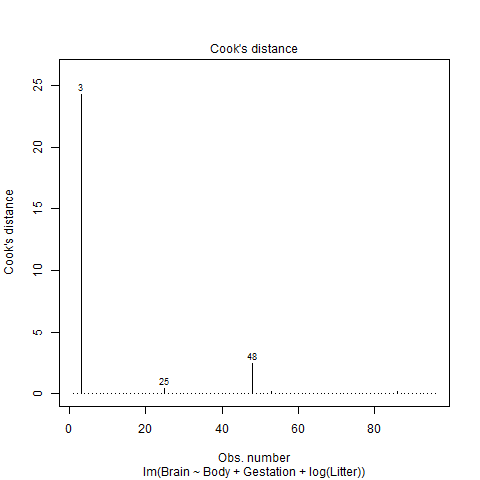
\includegraphics[scale= 0.6]{3_a_1.png}\\
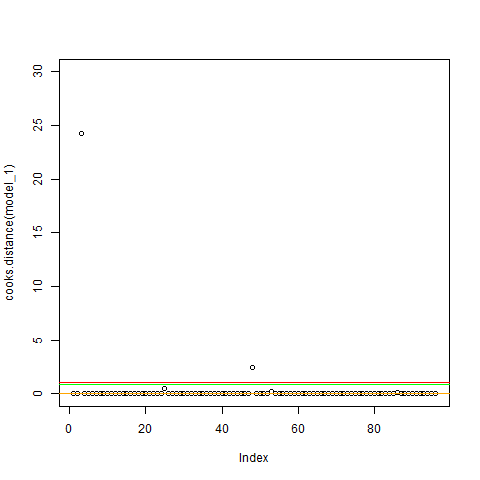
\includegraphics[scale=0.6]{3_a_2.png}\\
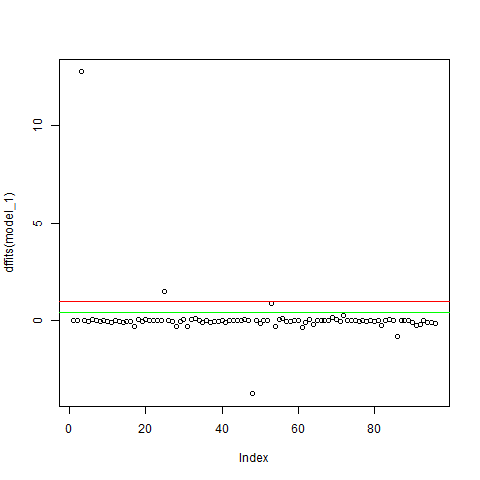
\includegraphics[scale=0.6]{3_a_3.png}
\end{center}
Based on the graphs, we can see that there are two influential points: 3, 25, 48, 53 and 86, which corresponding to African elephant, dolpin, hippopotamus, human being and Tapir respectively.
\subparagraph{(b)}~{}
After deleting the influential points, we do the regression again and get
\[Y = -135.44 + 0.47X_1 + 1.972X_2 + 39.38ln(X_3)\]
To find influential points, we compute the cook's distance and diffits value and the graphs are shown below:\\
\begin{center}
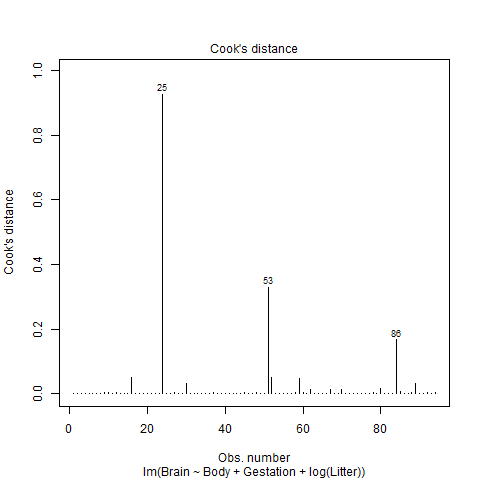
\includegraphics[scale= 0.6]{3_b_1.png}\\
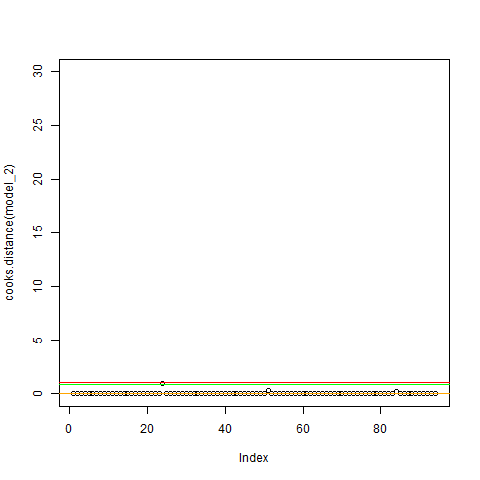
\includegraphics[scale=0.6]{3_b_2.png}\\
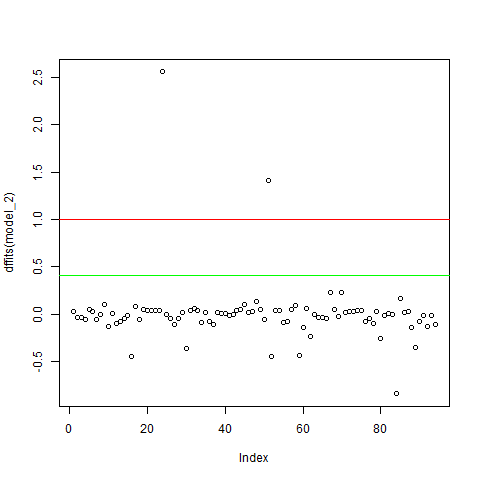
\includegraphics[scale=0.6]{3_b_3.png}
\end{center}
Based on the graphs, there are still  two influential points; 25 and 53.\\
\newline
Main differences: The coefficient of body weight and litter size and interception changed, F-value and t-value are decreasing.
\subparagraph{(c)}~{}
 Consider all the data and fit the regression of log brain weight on log body weight, log gestation, and log litter size:
\[ln(Y) = 0.85482 + 0.57507ln(X_1) + 0.41794ln(X_2) - 0.31007ln(X_3)\]
Then, we can calculate the studentized residuals:\\
\begin{center}
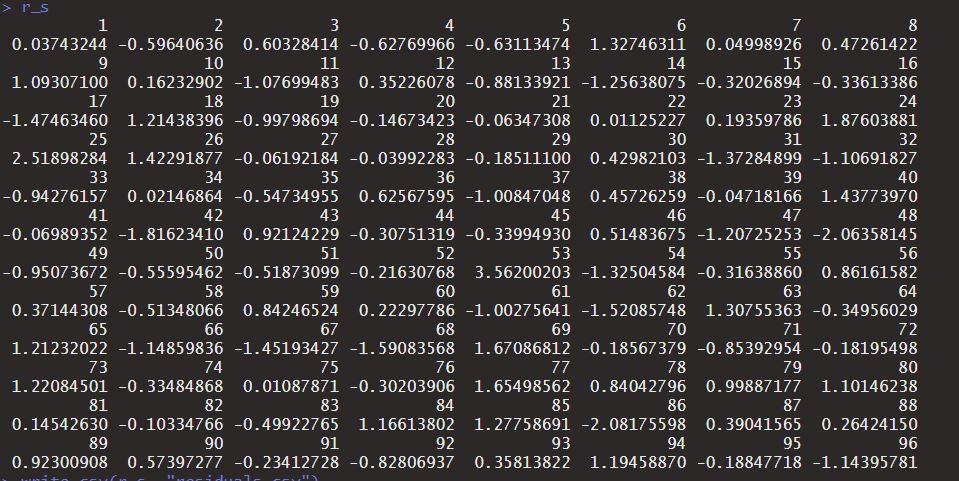
\includegraphics[scale = 0.6]{3_c.jpeg}
\end{center}
\subparagraph{(d)}~{}
To find influential points, we compute the cook's distance and fiffits value and the graphs are shown below:\\
\begin{center}
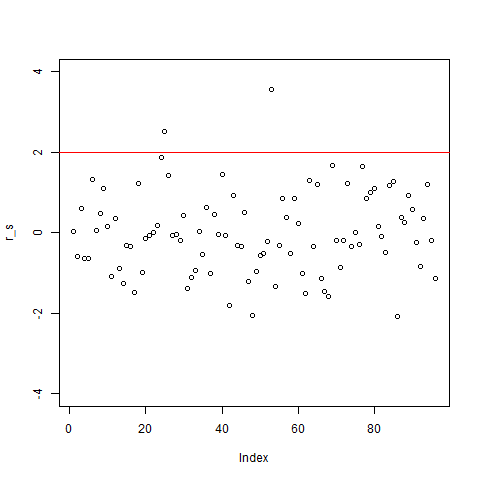
\includegraphics[scale=0.6]{3_d.png}
\end{center}
we can conclude that at the points 25 and 53, which corresponding to dolphin and human, have substantially larger brain weights than were predicted by the model.
\subparagraph{(e)}~{}
According to the graphics shown in (d), the conclusion is --- there is no mammals have substantially smaller brain weights than were predicted by the model.
\subparagraph{(f)}~{}
\begin{enumerate}
\item
After log transformation, F-value increased, which means the model fits better.
\item
Removing influential points and refit the regression may not be a good way to make thing right, even make it worse.
\item
The assumption of normality can hold by log transformation.
\end{enumerate}
\paragraph{Problem 4}
\subparagraph{(a)}
SSTO = 8100 and $\hat{\sigma^2} = \frac{SSE}{df}$. The estimates of $\sigma^2$ are shown below:\\
\begin{center}
\begin{tabular}{|l|l|}
\hline
Model variables & $\hat{\sigma}^2$ \\ \hline
None            & 300      \\ \hline
A               & 240        \\ \hline
B               & 230        \\ \hline
C               & 260        \\ \hline
AB              & 220      \\ \hline
AC              & 210      \\ \hline
BC              & 230      \\ \hline
ABC             & 215      \\ \hline
\end{tabular}
\end{center}
\subparagraph{(b)}~{}
Adjusted $R^2 = 1 - \frac{\frac{SSE_p}{n - p}}{\frac{SSTO}{N - 1}}$. The adjusted $R^2$ are shown below:\\
\begin{center}
\begin{tabular}{|l|l|}
\hline
Model variables &  Adjusted $R^2$ \\ \hline
None            & 0      \\ \hline
A               & 0.2        \\ \hline
B               & 0.233        \\ \hline
C               & 0.133      \\ \hline
AB              & 0.267      \\ \hline
AC              & 0.3      \\ \hline
BC              & 0.233      \\ \hline
ABC             & 0.283      \\ \hline
\end{tabular}
\end{center}
\subparagraph{(c)}~{}
$C_p(M) = \frac{SSE(M)}{\hat{\sigma}^2} - n + 2p(M)$, the $C_p$ statistics are shown below:\\
\begin{center}
\begin{tabular}{|l|l|}
\hline
Model variables &  $C_p$ \\ \hline
None            & 11.674      \\ \hline
A               & 5.023        \\ \hline
B               & 3.814        \\ \hline
C               & 7.442      \\ \hline
AB              & 3.851     \\ \hline
AC              & 2.419     \\ \hline
BC              & 4.744     \\ \hline
ABC             & 4      \\ \hline
\end{tabular}
\end{center}
\subparagraph{(d)}~{}
$BIC_p = nln(SSE_p) - nln(n) + pln(n)$. The $BIC$ are shown below:\\
\begin{center}
\begin{tabular}{|l|l|}
\hline
Model variables &  $BIC_p$ \\ \hline
None            & 162.0198      \\ \hline
A               & 158.0473        \\ \hline
B               & 156.8556        \\ \hline
C               & 160.2885      \\ \hline
AB              & 157.8450      \\ \hline
AC              & 156.5424     \\ \hline
BC              & 159.0896      \\ \hline
ABC             & 159.3905      \\ \hline
\end{tabular}
\end{center}
\subparagraph{(e)}~{}
\newline
(i)The last model with variables A, B and C has the smallest $\hat{\sigma}^2$, 198.46.\\
\newline
(ii)The model with variables A and C has the largest adjusted $R^2$, 0.3.\\
\newline
(iii)The model with variables A and C has the smallest $C_p$ statistic, 2.419.\\
\newline
(iv)The model with variables A and C has the smallest $BIC$, 156.54.\\
\subparagraph{(f)}~{}
\newline
Starting with none variable, we get the model contains Bhas the smallest SSE. Then we perform an extra-sum-of-squares F -test to see whether that variable is significant.\\
\newline
Under $\alpha = 0.05$, $F =7.75$. Thus, B is significant. \\
\newline
Then, we get AB has the smaller SSE. Samely, we perform an extra-sum-of-squares F -test to see whether the additional variable is significant. \\
\newline
Under $\alpha = 0.05$, $F = 2.182 < 4.24 = F_{1, n - 4, 0.05}$. So Ais insignificant.\\
\newline
Finally, by forward selecion, we have the model form:\[Y  \beta_0 + \beta_2B + \epsilon\]
\subparagraph{(g)}~{}
To find the posterior probability for these 8 models, we first subtract the smallest BIC from the other ones, and then calculate the difference of each model as below:\[BIC^*_j = BIC_j - BIC_{min}\]
Then,we have the posterior probability:
\[p(M_j) = \frac{e^{-\frac{1}{2}BIC^*_j}}{\sum^k_{j = 1}e^{-\frac{1}{2}BIC^*_j}}\]
The posterior distributions are shown below:
\begin{center}
\begin{tabular}{|l|l|}
\hline
Model variables &  Posterioir distribution \\ \hline
None            &    0.01802701    \\ \hline
A               & 0.13138647         \\ \hline
B               & 0.23840663       \\ \hline
C               & 0.04284313     \\ \hline
AB              & 0.14537115     \\ \hline
AC              & 0.27882110    \\ \hline
BC              & 0.07802002    \\ \hline
ABC             & 0.06712450   \\ \hline
\end{tabular}
\end{center}
\appendix
\section{Appendix: Problem 2}
\begin{lstlisting}[language = R]
bats = read.csv( file = "bats.csv" , header = T) 
bats = transform(bats , lenergy = log(Energy)) 
bats = transform(bats , lmass = log(Mass)) 
lm1 = lm(lenergy ~ lmass , data = bats) 
lm2 = lm(lenergy ~ lmass + Type, data = bats) 
lm3 = lm(lenergy ~ Type*lmass , data = bats)
anova(lm1,lm2,lm3)
\end{lstlisting}
\section{Appendix: Problem 3}
\begin{lstlisting}[language = R]
data = read.csv( "brain.csv")
model_1=lm(Brain ~ Body+Gestation+log(Litter) ,data = data) 
summary(model_1) 
cooks.distance(model_1) 
n = dim(model.matrix(model_1))[1] 
p = dim(model.matrix(model_1))[2] 
png("3_a_1.png") 
plot(model_1, which = 4) 
dev.off () 
png( "3_a_2.png")
plot(cooks.distance(model_1)  ,ylim = c (0,30)) 
abline(h=1, col="red") 
abline(h=qf (0.5 , p, n-p) , col="green") 
abline(h=4/n, col="blue") 
abline(h=4/(n-p-1-1), col="orange") 
dev.off () 
dffits (model_1)
png("3_a_3.png")
plot( dffits (model_1) ) 
abline(h=1, col="red") 
abline(h=2*sqrt(p/n) , col="green") 
dev.off () 
summary(influence.measures(model_1)) 
data_new = data[-48,][-3,]
model_2=lm(Brain ~ Body+Gestation+log(Litter) ,data = data_new) 
summary(model_2) 
cooks.distance(model_2) 
n = dim(model.matrix(model_2))[1] 
p = dim(model.matrix(model_2))[2] 
png("3_b_1.png") 
plot(model_2, which = 4) 
dev.off () 
png( "3_b_2.png")
plot(cooks.distance(model_2)  ,ylim = c (0,30)) 
abline(h=1, col="red") 
abline(h=qf (0.5 , p, n-p) , col="green") 
abline(h=4/n, col="blue") 
abline(h=4/(n-p-1-1), col="orange") 
dev.off () 
dffits (model_2)
png("3_b_3.png")
plot( dffits (model_2) ) 
abline(h=1, col="red") 
abline(h=2*sqrt(p/n) , col="green") 
dev.off () 
summary(influence.measures(model_2)) 
\end{lstlisting}
\end{document}